\hypertarget{part-2-image-3}{%
	\section{Part 2, Image 3}\label{part-1-design-2}}

\centering


\hypertarget{description}{%
	\subsubsection{Description}\label{description}}

\begin{description}
	\item[Image:]
	
	\item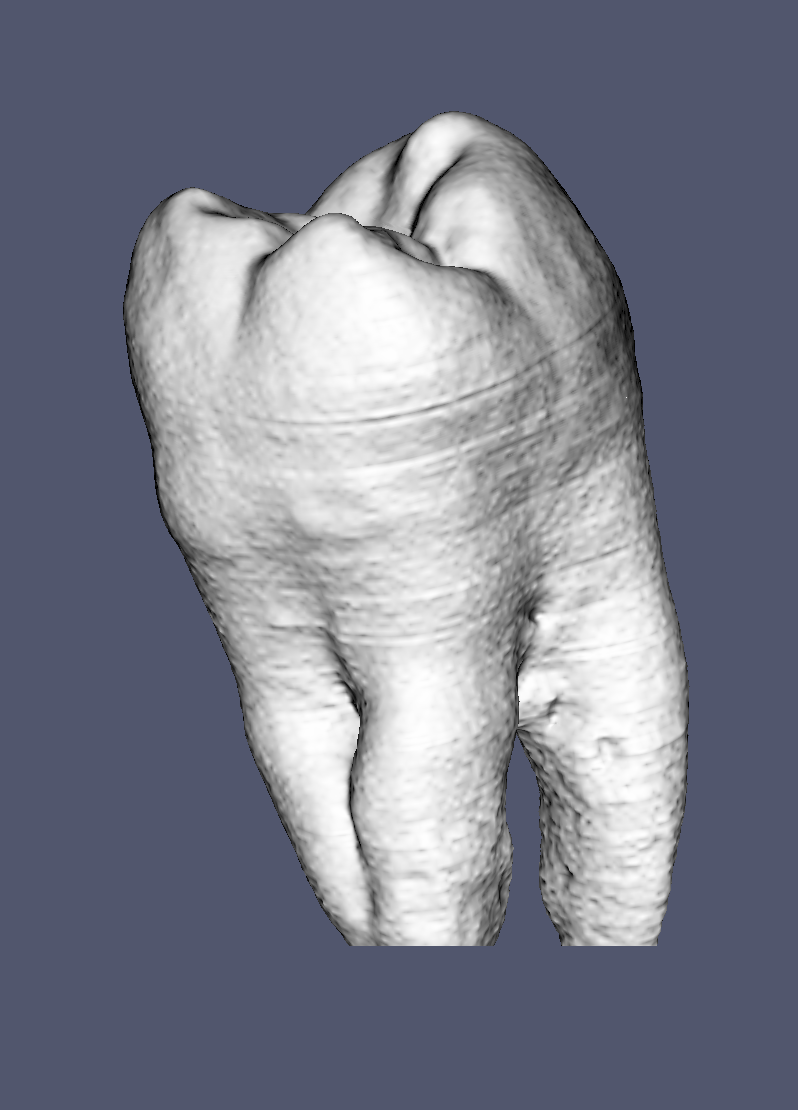
\includegraphics[width=9cm]{Tooth3.png}
	
	\item[Tool:]
	\hfill \break
		Paraview
	
	\item[Visual Mappings:]
	\begin{itemize}
		\tightlist
		\item[ ]
	\end{itemize}
	
	\begin{itemize}
		\tightlist
		\item
		\textbf{Mapping 1}: 
		\hfill \break
			Colour is set to X-ray with a colour space of RGB and a nan opacity of 1.
	\end{itemize}
	
	\begin{itemize}
		\tightlist
		\item
		\textbf{Mapping 2}: 
		\hfill \break
			At data point 650 the colour mapping starts at white with an opacity of 0.000, with a linear increase to 1300.00 at opacity 1.000. At data point 1160.642, this is where the change from white to black happens.
	\end{itemize}
	
	\item[Data Conversion:] 
	\hfill \break
		Data scalar type unsigned short was used with a representation of volume used. Volume rendering was set to OSPRay Based and a blend mode set to Isosurface. Data extent: 0 - 511, 0 - 511, 0 - 181 was used and data byte order of BigEndian.
	
	\item[Unique Observation:]
	\hfill \break
		A full tooth and roots are displayed with the tooth bite grooves. The data value 650 shows the outside Isosurface layer that creates the outside layer of the tooth.
	
\end{description}